\section{\texorpdfstring{Core Framework: The Coherence Field $\Xi$}{Core Framework: The Coherence Field Xi}}


At the foundation of General Coherence Field Theory (GCFT) lies a single continuous complex field, $\Xi$, which spans all of spacetime and encodes coherence phase, compression, and torsion at every point. Unlike quantum field theory (QFT), which begins with a vacuum populated by quantized excitations, GCFT postulates only one field — the coherence field~$\Xi$ — whose geometric and dynamical structure gives rise to all known matter and interactions.

\subsection{Field Properties and Structure}

The coherence field~$\Xi$ is modeled as a complex-valued scalar field with real-valued spatial phase structure. Its observable properties emerge from:

\begin{itemize}
    \item \textbf{Phase topology} ($\arg(\Xi)$): Encodes resonance structure, curvature, and oscillation patterns.
    \item \textbf{Compression modulus} ($|\Xi|$): Represents local coherence density. Gradients in $|\Xi|$ correspond to compressive tension and gravitational effects.
    \item \textbf{Phase torsion} ($\nabla \times \nabla \arg(\Xi)$): Captures chirality, circulation, and magnetic-like effects.
\end{itemize}

These elements allow mass, spin, charge, and even gravity to emerge as expressions of internal configurations within~$\Xi$, without requiring independent quantum fields or particles.

\subsection{Foundational Structures: Luxion, Xion, and Creaton}

GCFT replaces the notion of fundamental particles with stable or metastable field structures:

\begin{itemize}
    \item \textbf{Luxion} — A pure phase ripple in~$\Xi$ that propagates without compression. It preserves coherence across space, functioning as the GCFT analog of the photon.
    \item \textbf{Xion} — A localized compression node in~$\Xi$, forming a locked resonance. It gives rise to mass-bearing structures such as electrons and protons.
    \item \textbf{Creaton} — A resonance ignition threshold: the point at which decoherent background transitions into a standing~$\Xi$-structure.
\end{itemize}

\begin{figure}[ht]
\centering
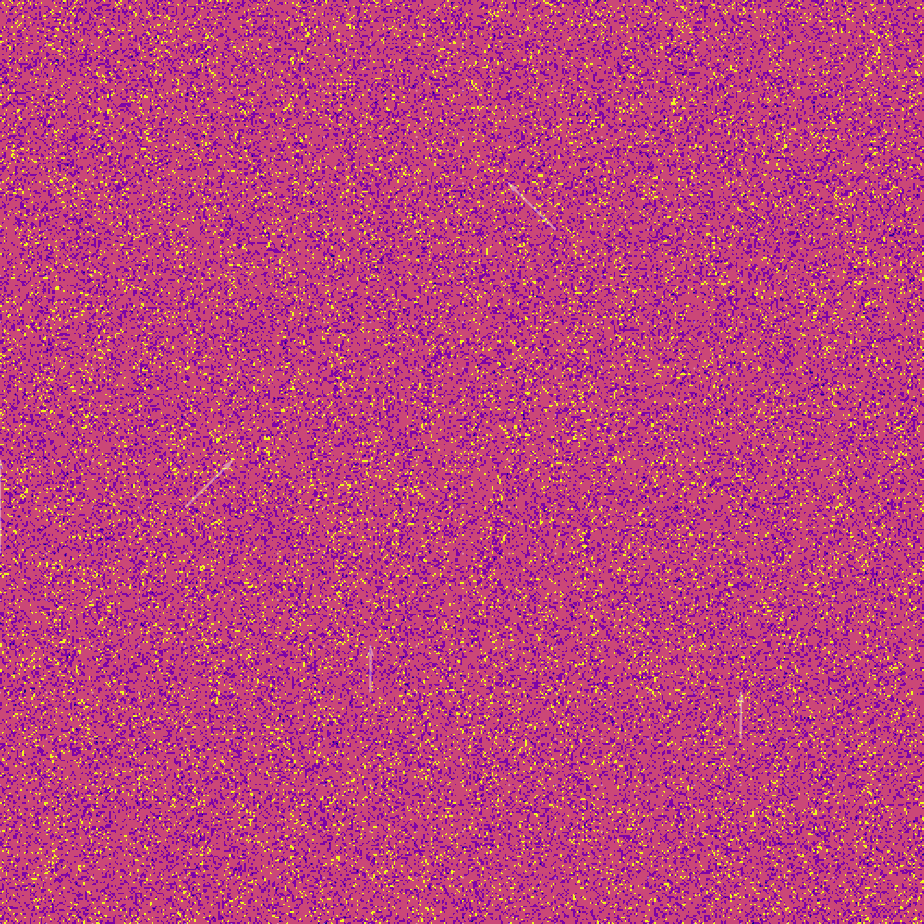
\includegraphics[width=0.48\textwidth]{figures/xi_photon_modulus_vector_overlay.png}
\caption{Luxion: a coherence-preserving wavefront in the $\Xi$-field. Field vectors flow continuously through the structure with no mass-lock, illustrating a pure phase carrier.}
\label{fig:xi_photon_phase}
\end{figure}

\begin{figure}[ht]
\centering
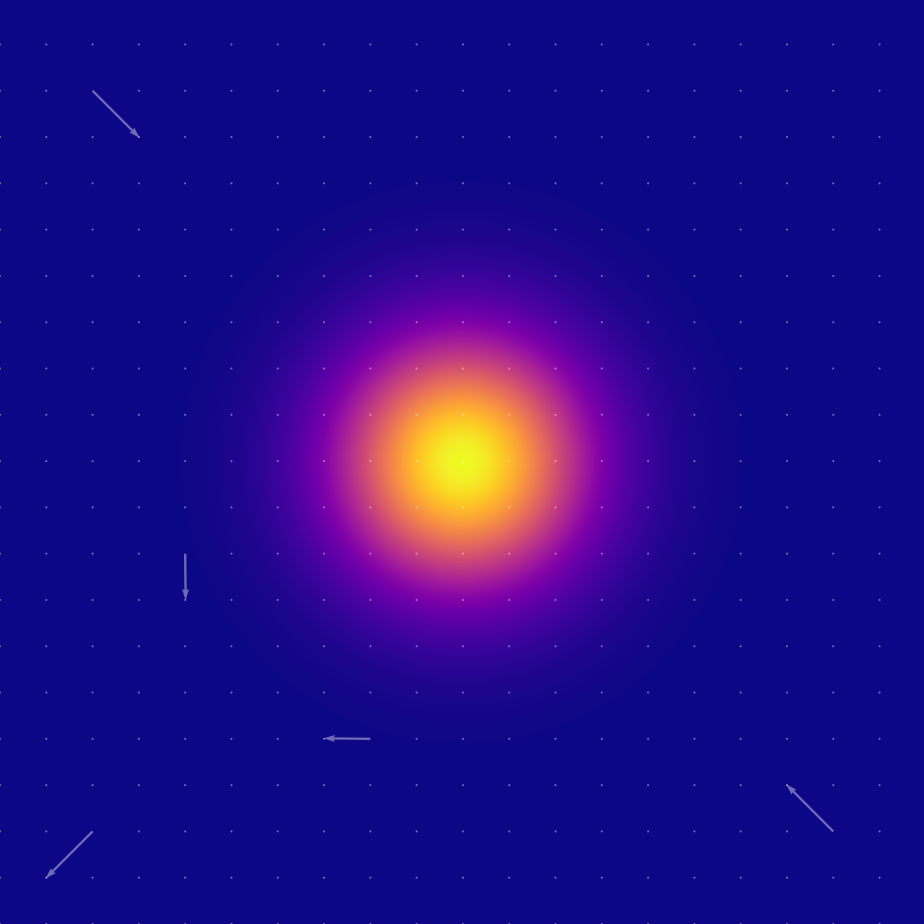
\includegraphics[width=0.48\textwidth]{figures/xi_core_modulus_vector_overlay.png}
\caption{Xion / Creaton: a localized compression node in the $\Xi$-field. This high-coherence structure locks phase and curvature, forming a stable resonance core associated with mass.}
\label{fig:xi_core_structure}
\end{figure}

\subsection{Topological Recursion and Particle Genesis}

In GCFT, all stable particles emerge from recursive self-structuring of~$\Xi$. Rather than relying on symmetry groups or quantized interactions, the theory models matter as attractors in a topological phase landscape, constrained by boundary conditions and compression thresholds. The coherence field retains phase memory and resonance curvature, enabling hierarchical structures to form from a single ontological substrate.
